\documentclass[a4paper,12pt]{article}

%% Language and font encodings
\usepackage[english]{babel}
\usepackage[utf8x]{inputenc}
\usepackage[T1]{fontenc}

%% Sets page size and margins
\usepackage[a4paper,top=2cm,bottom=2cm,left=3cm,right=3cm,marginparwidth=1.75cm]{geometry}

%% Useful packages
\usepackage{textcomp}
\usepackage{amsmath}
\usepackage{mathtools}
\usepackage{graphicx}
\usepackage{bigstrut}
\usepackage{numprint}
\usepackage{color}
\usepackage{float}
\usepackage[figurename=Figura]{caption}
\usepackage[tablename=Tabella]{caption}

\title{Grafi e Componenti Fortemente Connesse}
\author{***}
\date{19 agosto 2017}

\begin{document}
\maketitle

\section{Introduzione}
\subsection{Grafi}
Un grafo è un insieme di elementi detti \textbf{vertici} (o nodi) che possono essere collegati fra di loro tramite linee chiamate \textbf{archi}. In particolare, si dice grafo la coppia ordinata di insiemi $G = (V, E)$, dove $V$ è l'insieme dei vertici di $G$ e $E$ è l'insieme degli archi di $G$.

Un grafo si dice \textbf{orientato} (o \textbf{diretto}) se $E$ è un insieme di archi \textit{orientati}, cioè con una direzione (da sorgente a destinazione). Viceversa, un grafo si dice \textbf{non orientato} (o \textbf{indiretto}) se gli archi non sono orientati, dunque se la connessione tra due vertici i\textrightarrow j ha lo stesso significato della connessione j\textrightarrow i.

\begin{figure}[h]
    \centering
    \captionsetup{justification=centering,margin=1cm}
    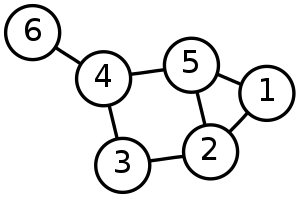
\includegraphics[width=0.4\textwidth]{graph}
    \caption{Un esempio di grafo indiretto con 6 vertici. [\textit{wikipedia.org}]}
    \label{fig:graph}
\end{figure}

\subsubsection{Rappresentazione}
Esistono due modalità per la rappresentazione di grafi tramite una struttura dati:
\newline

- \textbf{Lista di adiacenza:}
si introduce un vettore $Adj$ composto da $|V|$ liste, una per ogni nodo, dove $Adj[u]$ contiene tutti i vertici $v$ t.c. $(u, v) \in E$.

La lista di adiacenza richiede uno spazio di memoria $\Theta(V + E)$, e un tempo $O(u.degree)$ per determinare se due vertici qualsiasi $(u, v) \in E$.

In questo caso $u.degree$ rappresenta il \textbf{grado} del vertice $u$, ovvero il numero di archi che incidono in $u$.
\newline

- \textbf{Matrice di adiacenza:}
si introduce una matrice A ($|V|\times|V|$), dove ogni elemento $(i, j)$ ha valore 1 se $(i, j) \in E$, cioè se il vertice $j$ è adiacente a $i$, e valore 0 altrimenti.

La matrice di adiacenza richiede uno spazio di memoria $\Theta(V^2)$, quindi peggiore rispetto alla lista, però consente di determinare se due vertici qualsiasi $(u, v) \in E$ in un tempo $\Theta(1)$ (è sufficiente accedere all'elemento $A[u][v]$ e controllarne il valore).

In generale, una matrice di adiacenza è più indicata per descrivere grafi densi e con molti archi, inoltre rende più facile invertire i grafi, operazione che viene richiesta nell'algoritmo di ricerca di componenti fortemente connesse.
\newline

Per gli esperimenti svolti in seguito è stata utilizzata esclusivamente la rappresentazione con \textit{matrice di adiacenza}.

\subsubsection{Componenti fortemente connesse}
Dato il grafo diretto $G = (V, E)$ una componente fortemente connessa (o, in inglese, \textit{strongly connected component}, scc) $G$ è un insieme massimale di vertici $C ⊆ V$ t.c. per ogni $u,v \in C$ esistono entrambi i cammini u\textrightarrow v e v\textrightarrow u.

\section{Analisi delle operazioni su grafi}
\subsection{Breadth-First Search (BFS)}
La ricerca in ampiezza (in inglese \textit{breadth-first search}, BFS) è un algoritmo di ricerca per grafi che scopre vertici raggiungibili da nodo sorgente $s \in V$.
\newline

In particolare, questo algoritmo prende in input un grafo $G = (V, E)$ e un nodo sorgente $s \in V$, e per ogni vertice $v \in V$ scopre la \textit{distanza} (numero minimo di archi) da $s$ a $v$ ed imposta il predecessore $u (v.\pi)$ di $v$.

L’insieme di archi ${(v.\pi, v) : v\neq s}$ forma un albero.

L'algoritmo utilizza una coda di tipo FIFO per la gestione dei nodi visitati o ancora da visitare.
\newline

Mentre l'algoritmo progredisce, ogni nodo possiede un colore specifico:\newline
- \textbf{White} (bianco): nodo non ancora scoperto.\newline
- \textbf{Gray} (grigio): nodo scoperto, ma non visitato.\newline
- \textbf{Black} (nero): nodo visitato.
\newline

Il tempo di esecuzione complessivo richiesto da $BFS$ è $O(V +E)$ ($O$ e non $\Theta$ perchè l'algoritmo può non raggiungere tutti i nodi).

\subsection{Depth-First Search (DFS)} \label{ssec:dfs}
La ricerca in profondità (in inglese \textit{depth-first search}, DFS) è un algoritmo di ricerca per grafi di tipo ricorsivo, di cui è stata fornita una implementazione nel file \textbf{dfs.py}.
\newline

In particolare, questo algoritmo prende in input un grafo $G = (V, E)$ ed esplora sistematicamente ogni suo vertice $v \in V$ determinandone il tempo di scoperta $(v.d)$, il tempo di fine $(v.f)$ e il predecessore $u (v.\pi)$ di $v$.

Come per il $BFS$, gni nodo può avere tre diversi colori (bianco, grigio, nero) in base allo stato in cui si trova; inizialmente tutti i vertici vengono colorati di bianco, e tutti predecessori vengono azzerati.
\newline

L'algoritmo in sè è suddiviso in due funzioni:
\newline

1) \textbf{DFS()}: è la procedura che avvia la ricerca: viene chiamata la funzione \textit{DFS-Visit(u)} per tutti i vertici $u \in V$ di colore bianco.

Questa procedura necessita di una modifica nel caso in cui l'esecuzione sia al passo 3 dell'algoritmo per trovare componenti fortemente connesse: in questo caso, prima di procedere alla chiamata di \textit{DFS-Visit(u)}, i vertici vengono ordinati in maniera decrescente rispetto al tempo di completamento $u.f$.
\newline

2) \textbf{DFS-Visit(u)}: tutte le volte che viene chiamata questa procedura, il vertice $u$ (inizialmente bianco) diventa la radice di un nuovo albero della foresta DF. Ogni vertice $v$ adiacente a $u$ viene poi ispezionato in modo ricorsivo se anch'esso è bianco. Infine il vertice $u$ viene colorato di nero e viene aggiornato il suo tempo di completamento.
\newline

Una volta completata la visita in profondità, il sottografo dei predecessori forma una foresta Depth-First contenente almeno un albero DF: questa proprietà risulta particolarmente utile per la scomposizione di un grafo orientato nelle sue componenti fortemente connesse (vedi \ref{ssec:scc}).
\newline

Il tempo di esecuzione complessivo richiesto da $DFS$ è $\Theta(V +E)$ ($\Theta$ e non $O$ perchè l'algoritmo esplora ogni nodo e arco).

\subsection{Strongly-Connected-Components} \label{ssec:scc}
Si tratta dell'algoritmo per trovare componenti fortemente connesse in un grafo orientato $G = (V, E)$, basato su due visite in profondità: una su $G$ e una su $G^T$. $G^T$ è chiamato \textbf{grafo trasposto} di $G$ ed è definito come $G^T = (V, E^T)$ dove $E^T = \{(u, v) : (v, u) \in E\}$ ($G^T$ essenzialmente è un grafo i cui archi hanno direzioni invertite rispetto a $G$).

Nel caso di rappresentazione tramite matrice di adiacenza, il calcolo del grafo trasposto è semplice e si riduce al calcolo della matrice di adiacenza trasposta.

Una possibile implementazione di questo algoritmo è stata fornita nel file \textbf{scc.py}.

L'algoritmo si divide in quattro passi:
\newline

1) Chiama $DFS(G)$ per calcolare i tempi di completamento per ciascun vertice.

2) Calcola il grafo trasposto $G^T$.

3) Chiama $DFS(G^T)$, ma nel ciclo principale di $DFS$, considera i vertici in ordine decrescente rispetto ai tempi di completamento calcolati in precedenza.

4) Genera l'output dei vertici di ciascun albero della foresta DF prodotta al passo 3 come una singola componente fortemente connessa.
\newline

Il tempo complessivo richiesto dall'algoritmo è $\Theta(V +E)$.

\clearpage
\section{Descrizione esperimenti e documentazione del codice}
Gli esperimenti sono stati svolti su un MacBook Pro con sistema operativo macOS Sierra, processore 2,6 GHz Intel Core i5 e 8 GB di RAM.
\newline
\newline
Eventuali numeri casuali sono stati generati dalla funzione \textit{randint()} importata dalla libreria \textit{random}. Per il calcolo del grafo trasposto è stata utilizzata la funzione \textit{transpose()} della libreria \textit{numpy}.
\newline
\newline
Il codice è articolato in sei file: \textbf{vertice.py, graph.py, dfs.py, scc.py, tests.py, exp.py}.

\subsection{Vertice.py}
Nel file \textbf{vertice.py} è stata implementata una semplice classe per rappresentare i vertici di un grafo, con i seguenti attributi:
\newline
- $numero$, un numero intero che identifica ogni vertice. \newline
- $colore$, una stringa che rappresenta il colore del vertice: può essere `W` (colore bianco), `G` (colore grigio) o `B` (colore nero). \newline
- $d$, un numero intero che rappresenta il tempo di scoperta del vertice. \newline
- $f$, un numero intero che rappresenta il tempo di completamento del vertice. \newline
- $predecessore$, un numero intero che rappresenta il vertice predecessore.

\subsection{Graph.py}
Nel file \textbf{graph.py} è stata fornita una implementazione dei grafi tramite \textbf{matrice di adiacenza}. Il numero di vertici viene passato nel costruttore, mentre la presenza di archi tra vertici è stabilita su base probabilistica attraverso un parametro intero $perc$ compreso tra 0 e 10 e preso in ingresso dalla funzione $matrice\_adiacenza()$.

Nello specifico, se $perc$ è zero c'è lo 0\% di possibilità di archi tra due vertici; al contrario se $perc$ è 10 si ha il 100\% di archi nel grafo.

\subsection{Dfs.py}
Nel file \textbf{dfs.py} è stato implementato l'algoritmo di \textit{Depth-First Search} (DFS) per la ricerca in profondità su grafi come descritto nella sottosezione \ref{ssec:dfs}.
\newline

Nel caso in cui l'esecuzione si trovi al passo 3 dell'algoritmo per trovare componenti fortemente connesse (\ref{ssec:dfs}), è stata implementata una funzione alternativa chiamata \textit{dfs\_scc()} che si basa su un'array di vertici presa in ingresso: prima azzera tutti gli attributi di tali vertici (colore, predecessore), poi li ordina in maniera decrescente rispetto ai loro tempi di completamento, e infine chiama la \textit{dfs()} originale con i nuovi vertici ordinati.

Eventuali informazioni sulle componenti fortemente connesse del grafo (come ad esempio i vertici appartenenti alla singola componente) vengono salvate in un dizionario chiamato \textit{dizionario\_scc}, mentre il numero di componenti fortemente connesse trovate in un grafo viene salvato in un intero chiamato \textit{numero\_di\_scc}.

\subsection{Scc.py}
Nel file \textbf{scc.py} è stato implementato l'algoritmo per la ricerca di componenti fortemente connesse in un grafo diretto (\textit{strongly-connected-components(G)}), come descritto nella sottosezione \ref{ssec:scc}.

Nel costruttore viene passato come parametro la matrice di adiacenza del grafo da analizzare, mentre la funzione \textit{scc()} esegue l'algoritmo e restituisce:
\newline
- Il numero di componenti fortemente connesse del grafo. \newline
- Un dizionario contenente i vertici di ciascun albero (componente fortemente connessa) della foresta DF prodotta dall'algoritmo.

\subsection{Tests.py}
Nel file \textbf{tests.py} sono stati implementati i seguenti esperimenti:
\newline

- E' stata misurato il numero di componenti fortemente connesse per grafi di dimensione crescente (da 1 fino a 50 massimi vertici), con probabilità di archi tra vertici fissata al 20\%.
\newline

- E' stata misurato il numero di componenti fortemente connesse per grafi di dimensione fissata a 5 vertici e con probabilità di archi tra vertici crescente (da 0\% al 100\%).
\newline

- E' stata misurato il numero massimo di vertici contenuti in una componente fortemente connessa per grafi di dimensione crescente, sempre con probabilità di archi tra vertici fissata al 20\%.
\newline

- Sono stati valutati i tempi di esecuzione dell'algoritmo per la ricerca di componenti fortemente connesse in un grafo diretto, al crescere delle dimensioni del grafo.
\newline

- Sono stati raccolti i dati riguardanti il numero di componenti fortemente connesse e il numero massimo di vertici contenuti in una componente fortemente connessa, per grafi di determinate dimensioni (5, 10 ,15, 20, 25, 30, 35, 40) e densità di archi (da 0\% a 100\%).

\subsection{Exp.py}
Nel file \textbf{exp.py} sono stati eseguiti i test descritti nel file \textbf{tests.py} e generati i grafici e tabelle corrispondenti, presentati di seguito.

\clearpage
\section{Presentazione dei dati sperimentali}

\subsection{Numero di componenti fortemente connesse per grafi di dimensione crescente con probabilita' di archi fissata}
\begin{figure}[h]
    \centering
    \captionsetup{justification=centering,margin=1cm}
    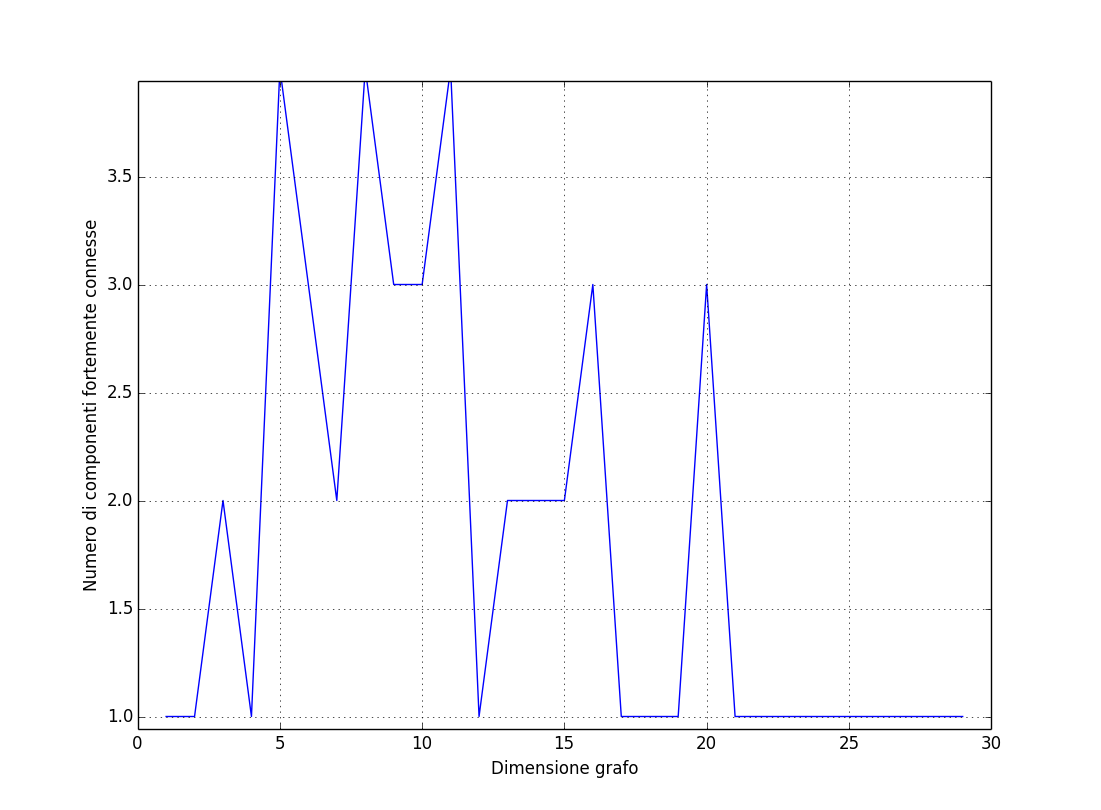
\includegraphics[width=1.0\textwidth]{test1}
    \caption{Variazione del numero di componenti fortemente connesse per grafi con un numero di vertici crescente e probabilita' di archi a 0.2.}
    \label{fig:test1}
\end{figure}

Per questo esperimento sono stati generati 30 grafi con dimensione da 1 a 30 (il primo di dimensione uno, il secondo di dimensione due ecc..). Per ognuno di questi grafi è stata generata una matrice di adiacenza con percentuale di archi tra vertici fissata al 20\%, e poi calcolato il numero di componenti fortemente connesse presenti.
\newline

Dal grafico generato si può notare come il numero di componenti fortemente connesse presenti un picco nelle dimensioni tra 5 e 20, poi si stabilizzi a 1 per dimensioni sempre maggiori.
\newline

Per motivi di semplicità il grafico è stato tagliato per mostrare soltanto le dimensioni da 1 a 30, ma in realtà dai test svolti di nota che qualsiasi grafo di dimensione superiore a 20 presenta una sola componente fortemente connessa (e questo vale prendendo in considerazione tutte le possibili percentuali di archi tra vertici, ad eccezione di quelle molto vicine allo 0\%).
\newline

Questo porta a concludere che maggiore è la dimensione del grafo, minore sarà il numero di componenti fortemente connesse.

\clearpage
\subsection{Numero di componenti fortemente connesse per grafi di dimensione fissata con probabilita' di archi crescente}
\begin{figure}[h]
    \centering
    \captionsetup{justification=centering,margin=1cm}
    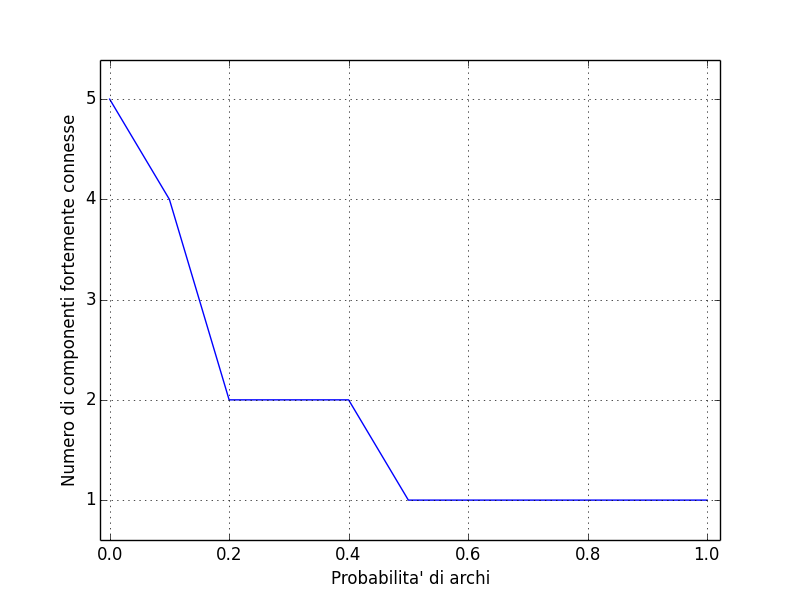
\includegraphics[width=1.0\textwidth]{test2}
    \caption{Variazione del numero di componenti fortemente connesse per grafi a 5 vertici e probabilita' di archi crescente.}
    \label{fig:test2}
\end{figure}

Per questo esperimento sono stati generati 11 grafi di dimensione fissata a 5 vertici, e per ognuno di questi è stata generata una matrice di adiacenza con percentuale di archi tra vertici crescente (il primo con probabilità 0\%, il secondo con probabilità 10\%, ecc...), e poi è stato calcolato il numero di componenti fortemente connesse presenti.
\newline

Dal grafico generato si può notare come il numero di componenti fortemente connesse in un grafo presenti un picco inziale, per poi stabilizzarsi a 1 per percentuali dal 50\% in poi.
\newline

In questo caso è stato scelto di fissare la dimensione dei grafi a 5 vertici, ma altri test secondari con dimensioni differenti hanno riportato un andamento molto simile.
\newline

Questo porta a concludere che maggiore è la densità del grafo (percentuale di archi tra vertici), minore sarà il numero di componenti fortemente connesse.

\clearpage
\subsection{Grandezza massima di componenti fortemente connesse per grafi di dimensione crescente e probabilita' di archi fissata}
\begin{figure}[h]
    \centering
    \captionsetup{justification=centering,margin=1cm}
    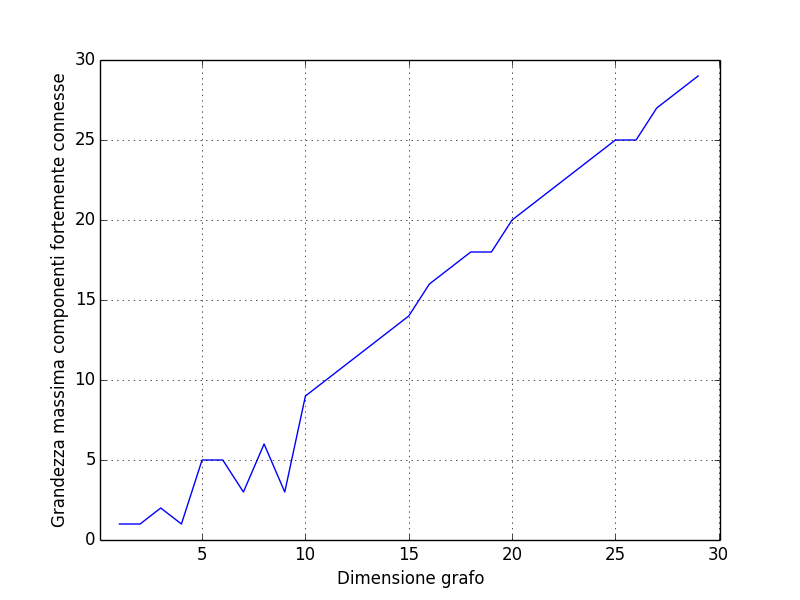
\includegraphics[width=1.0\textwidth]{test3}
    \caption{Variazione della grandezza massima di componenti fortemente connesse per grafi con un numero di vertici crescente e probabilita' di archi a 0.2.}
    \label{fig:test3}
\end{figure}

Per questo esperimento sono stati generati 30 grafi con dimensione da 1 a 30 (il primo di dimensione uno, il secondo di dimensione due ecc..). Per ognuno di questi grafi è stata generata una matrice di adiacenza con percentuale di archi tra vertici fissata al 20\%, e poi calcolata la grandezza massima di ogni componente fortemente connessa.
\newline

Dal grafico generato si può notare come la grandezza massima di componenti fortemente connesse in un grafo cresca in maniera lineare, di pari passo con la dimensione del grafo.
\newline

Questo porta a concludere che esiste una proporzionalità diretta tra la dimensione del grafo e il volume (grandezza massima) delle componenti fortemente connesse.

\clearpage
\subsection{Tempi di esecuzione dell'algoritmo per trovare componenti fortemente connesse per grafi di dimensione crescente e probabilita' di archi fissata}
\begin{figure}[h]
    \centering
    \captionsetup{justification=centering,margin=1cm}
    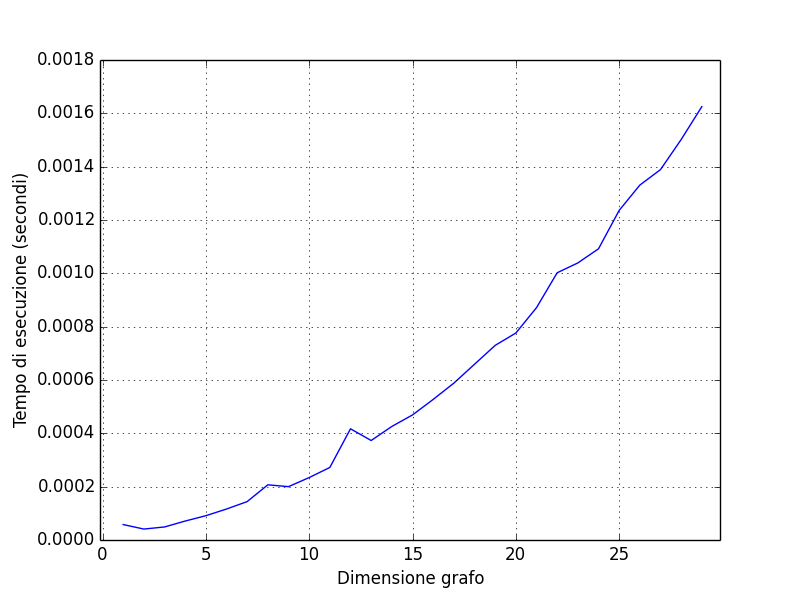
\includegraphics[width=1.0\textwidth]{test4}
    \caption{Variazione dei tempi di esecuzione dell'algoritmo per trovare componenti fortemente connesse per grafi con un numero di vertici crescente e probabilita' di archi a 0.2.}
    \label{fig:test4}
\end{figure}

Per questo esperimento sono stati generati 30 grafi con dimensione da 1 a 30 (il primo di dimensione uno, il secondo di dimensione due ecc..). Per ognuno di questi grafi è stata generata una matrice di adiacenza con percentuale di archi tra vertici fissata al 20\%, e poi calcolato il tempo di esecuzione dell'algoritmo per trovare le componenti fortemente connesse presenti.
\newline

Dal grafico generato si può confermare che l'algoritmo $SCC$ per trovare le componenti fortemente connesse in un grafo richieda un tempo complessivo lineare ($\Theta(V +E)$), come visto nella sottosezione \ref{ssec:scc}.

\clearpage
\section{Conclusioni}\label{ssec:con}
In conclusione, alla luce degli esperimenti svolti, si può affermare che \textbf{all'aumentare dell'ampiezza e della densità del grafo diminuiscono le componenti fortemente connesse ma aumenta il loro volume}.
\newline

L'unica eccezione avviene nel caso limite, ovvero quello in cui si ha densità molto vicina allo zero e dunque il numero di componenti fortemente connesse è sempre uguale al numero di vertici, ed ogni componente ha volume unitario (l'albero associato contiene soltanto il proprio vertice).
\newline

Questo è evidente anche dai dati raccolti dall'ultimo esperimento, presentati di seguito nelle tabelle \ref{tab:tab1} e \ref{tab:tab2}.

\begin{center}
\vspace*{0.9cm}
\begin{tabular}{|c|c|c|c|c|c|c|c|c|c|c|c|}
\hline
& \textbf{0.0}\bigstrut & \textbf{0.1} & \textbf{0.2} & \textbf{0.3} & \textbf{0.4} & \textbf{0.5} & \textbf{0.6} & \textbf{0.7} & \textbf{0.8} & \textbf{0.9} & \textbf{1.0} \\\hline
\textbf{5}\bigstrut & 5 & 4 & 3 & 2 & 1 & 3 & 1 & 1 & 1 & 1 & 1 \\\hline
\textbf{10}\bigstrut & 10 & 6 & 2 & 2 & 2 & 1 & 1 & 1 & 1 & 1 & 1 \\\hline
\textbf{15}\bigstrut & 15 & 2 & 1 & 1 & 1 & 1 & 1 & 1 & 1 & 1 & 1 \\\hline
\textbf{20}\bigstrut & 20 & 1 & 2 & 1 & 1 & 1 & 1 & 1 & 1 & 1 & 1 \\\hline
\textbf{25}\bigstrut & 25 & 4 & 1 & 1 & 1 & 1 & 1 & 1 & 1 & 1 & 1 \\\hline
\textbf{30}\bigstrut & 30 & 2 & 1 & 1 & 1 & 1 & 1 & 1 & 1 & 1 & 1 \\\hline
\textbf{35}\bigstrut & 35 & 4 & 1 & 1 & 1 & 1 & 1 & 1 & 1 & 1 & 1 \\\hline
\textbf{40}\bigstrut & 40 & 3 & 1 & 1 & 1 & 1 & 1 & 1 & 1 & 1 & 1 \\\hline
\end{tabular}
\captionsetup{justification=centering,margin=1.05cm}
\captionof{table}{La tabella mostra il numero di componenti fortemente connesse presenti nei grafi generati con deteminata dimensione (righe) e probabilità di archi tra vertici (colonne).}
\label{tab:tab1}
\end{center}

\begin{center}
\vspace*{0.7cm}
\begin{tabular}{|c|c|c|c|c|c|c|c|c|c|c|c|}
\hline
& \textbf{0.0}\bigstrut & \textbf{0.1} & \textbf{0.2} & \textbf{0.3} & \textbf{0.4} & \textbf{0.5} & \textbf{0.6} & \textbf{0.7} & \textbf{0.8} & \textbf{0.9} & \textbf{1.0} \\\hline
\textbf{5}\bigstrut & 1 & 2 & 3 & 5 & 4 & 5 & 5 & 5 & 5 & 5 & 5 \\\hline
\textbf{10}\bigstrut & 1 & 2 & 10 & 10 & 10 & 10 & 10 & 10 & 10 & 10 & 10 \\\hline
\textbf{15}\bigstrut & 1 & 11 & 12 & 15 & 15 & 15 & 15 & 15 & 15 & 15 & 15 \\\hline
\textbf{20}\bigstrut & 1 & 11 & 20 & 20 & 20 & 20 & 20 & 20 & 20 & 20 & 20 \\\hline
\textbf{25}\bigstrut & 1 & 22 & 25 & 25 & 25 & 25 & 25 & 25 & 25 & 25 & 25 \\\hline
\textbf{30}\bigstrut & 1 & 29 & 30 & 30 & 30 & 30 & 30 & 30 & 30 & 30 & 30 \\\hline
\textbf{35}\bigstrut & 1 & 33 & 35 & 35 & 35 & 35 & 35 & 35 & 35 & 35 & 35 \\\hline
\textbf{40}\bigstrut & 1 & 39 & 40 & 40 & 40 & 40 & 40 & 40 & 40 & 40 & 40 \\\hline
\end{tabular}
\captionsetup{justification=centering,margin=1.05cm}
\captionof{table}{La tabella mostra il volume massimo delle componenti fortemente connesse presenti nei grafi generati con deteminata dimensione (righe) e probabilità di archi tra vertici (colonne).}
\label{tab:tab2}
\end{center}

\end{document}
